
\section{\lsystem processing library}

Main design goal of \lsystem processing library is simple extensibility.
It should be possible to alter processing of \lsystem without need of changing whole process system.
This behavior is achieved by modular design -- input is processed with set of connected components.
Each component is specialized for one activity for example symbol rewriting or rendering of image.
Both components and connections are definable by user.

Component-based modular system have many advantages over monolithic system.
Probably the biggest and already discussed advantage is easy extensibility.
It is simple to implement extension component and include it into system.
Also it is possible to improve existing components and extend system capabilities.
Simple illustration of component system extension is shown in Figure \ref{fig:extensionExample}, system \ref{fig:extensionExampleBase} was extended by gravity simulation component to system \ref{fig:extensionExampleExtended}.
Possible results are in Figure \ref{fig:extensionExampleResult}.

Another advantage lies in specialization of components.
Specialized components are easier to implement and result will likely have less bugs.
Specialization also helps system robustness because individual components can be tested separately.
Tests for single component are easier to write and they can test situations which can not be tested on whole system.

\begin{figure}[h]
	\centering
	\subfloat[Simple component-based system]{
		\begin{tikzpicture}[auto, node distance=4cm,>=latex]
			\node (in) [coord] {};
			\node (rw) [block, right of=in, node distance=3cm] {Rewriter};
			\node (int) [block, right of=rw] {Interpreter};
			\node (out) [coord, right of=int, node distance=3cm] {};
			
			\draw [->] (in) -- node {input} (rw);
			\draw [->] (rw) -- node {} (int);
			\draw [->] (int) -- node {output} (out);
		\end{tikzpicture}
		\label{fig:extensionExampleBase}
	}
	\\
	\subfloat[Extended component-based system]{
		\begin{tikzpicture}[auto, node distance=4cm,>=latex]
			\node (in) [coord] {};
			\node (rw) [block, right of=in, node distance=3cm] {Rewriter};
			\node (g) [blockx, right of=rw] {Gravity simulation};
			\node (int) [block, right of=g] {Interpreter};
			\node (out) [coord, right of=int, node distance=3cm] {};
			
			\draw [->] (in) -- node {input} (rw);
			\draw [->] (rw) -- node {} (g);
			\draw [->] (g) -- node {} (int);
			\draw [->] (int) -- node {output} (out);
		\end{tikzpicture}
		\label{fig:extensionExampleExtended}
	}
	\caption{Example of extension of component-based \lsystem processing system}
	\label{fig:extensionExample}
\end{figure}

\begin{figure}[h]
	\centering
	\subfloat[Original tree model (no effect of gravity)]{
		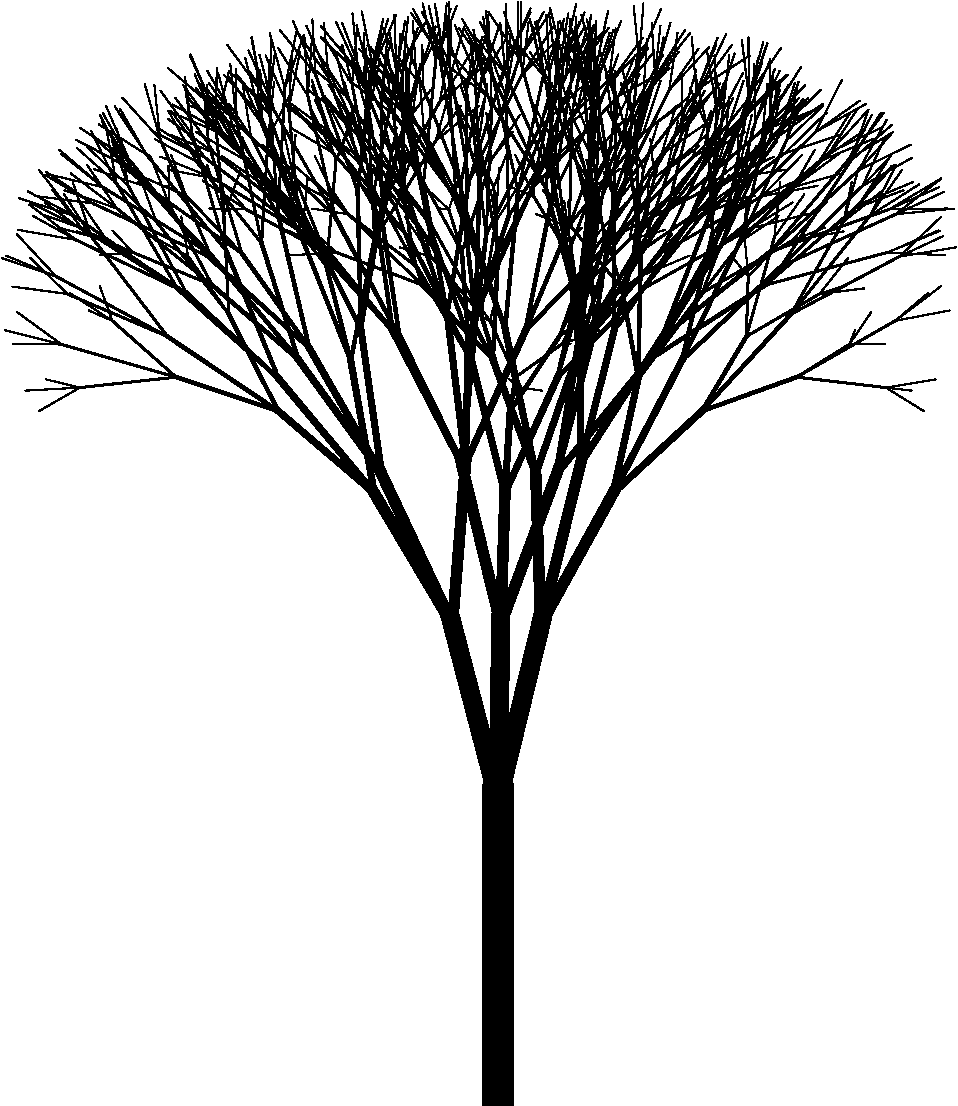
\includegraphics[scale=0.4]{ComponentSystemGravityOff}
	} ~
	\subfloat[Tree model with simulated gravity]{
		
\includegraphics[scale=0.4]{ComponentSystemGravityOn}
	}
	\caption{Possible outputs from process systems in Figure \ref{fig:extensionExample}}
	\label{fig:extensionExampleResult}
\end{figure}


\subsection{Input form}

Input is important part of application.
\lsystems have no standardized input for example like programming languages.
Every implementation of \lsystem processor uses its own variant of input.

Main goals for input design are simplicity and universality.
With simple input there is lower barrier for new user to start using the application.
Complicated input might discourage many potential users.
Universal input means that \textit{everything} is possible to define by input including definitions of \lsystems, configuration of components, etc.

Generally there are two basic types of input, graphic interface and source code.
Source code was chosen as input because it is better for saving, sharing and versioning.
Statements can be easily commented thus ideas behind code can be saved with it.
Parts of code can be copy-pasted and the syntax can be extended.
Parsing of source code is quite complex but input interface can be just one text area.

%Graphic interface is better for new users.
%Values are written in text boxes and chosen from select boxes so it easier to create valid input.
%Also parsing of input is easier because values are separated by user.
%On the other hand implementation of well-arranged graphic interface for complex system can be very hard and time-consuming.

To achieve good readability of input source code the syntax will be rich on keywords.
This should ensure that even new users will understand the statements.
With source code input it is still possible to create second type of input -- the graphic interface.
It can be achieved by source code designers but this will be left as future extension.


\subsection{What is described by input}

The goal of input design is to be able to describe everything by it.
By everything is meant \lsystem definitions, configuration of components, definitions of component systems, what \lsystem process with what component system etc.
This is important for easy saving and sharing.

Following list describes concrete entities which are possible to describe with source code.
Full reference of input syntax is in appendix \ref{chap:syntax}.
Small example of input source code together with the result is shown in Figure \ref{fig:scExample}.

\begin{itemize*}
	\item Global constant
	\item Global function
	\item \lsystem definition
		\begin{itemize*}
			\item Local constant
			\item Local function
			\item Component property assign
			\item Component symbol property assign
			\item Symbol interpretation -- defined interpretation for one or more \lsystem symbols
			\item Rewrite rule
		\end{itemize*}
	\item Process configuration -- definition of component system
		\begin{itemize*}
			\item Component
			\item Container -- components in container can be reassigned when \lsystem is processed by process configuration
			\item Connection -- defines connection between two components
		\end{itemize*}
	\item Process statement -- defines processing of \lsystem with process configuration
		\begin{itemize*}
			\item Container component reassign -- change of component in container
			\item Additional \lsystem statements -- additional \lsystem statements which can alter processed \lsystem
		\end{itemize*}
\end{itemize*}

\newsavebox{\lstBox}
\begin{lrbox}{\lstBox}
\begin{Lsystem50}
lsystem SierpinskiGasket {
	set symbols axiom = + R;
	set iterations = 7;

	interpret L R as DrawForward(
		2 ^ -currentIteration
		* 700);
	interpret + as TurnLeft(60);
	interpret - as TurnLeft(-60);

	rewrite L to R + L + R;
	rewrite R to L - R - L;
}
process all with SvgRenderer;
\end{Lsystem50}
\end{lrbox}

\begin{figure}[h!]
	\subfloat{
		\usebox{\lstBox}
	} \hfill
	\subfloat{
		\minipage{0.47\linewidth}\noindent
		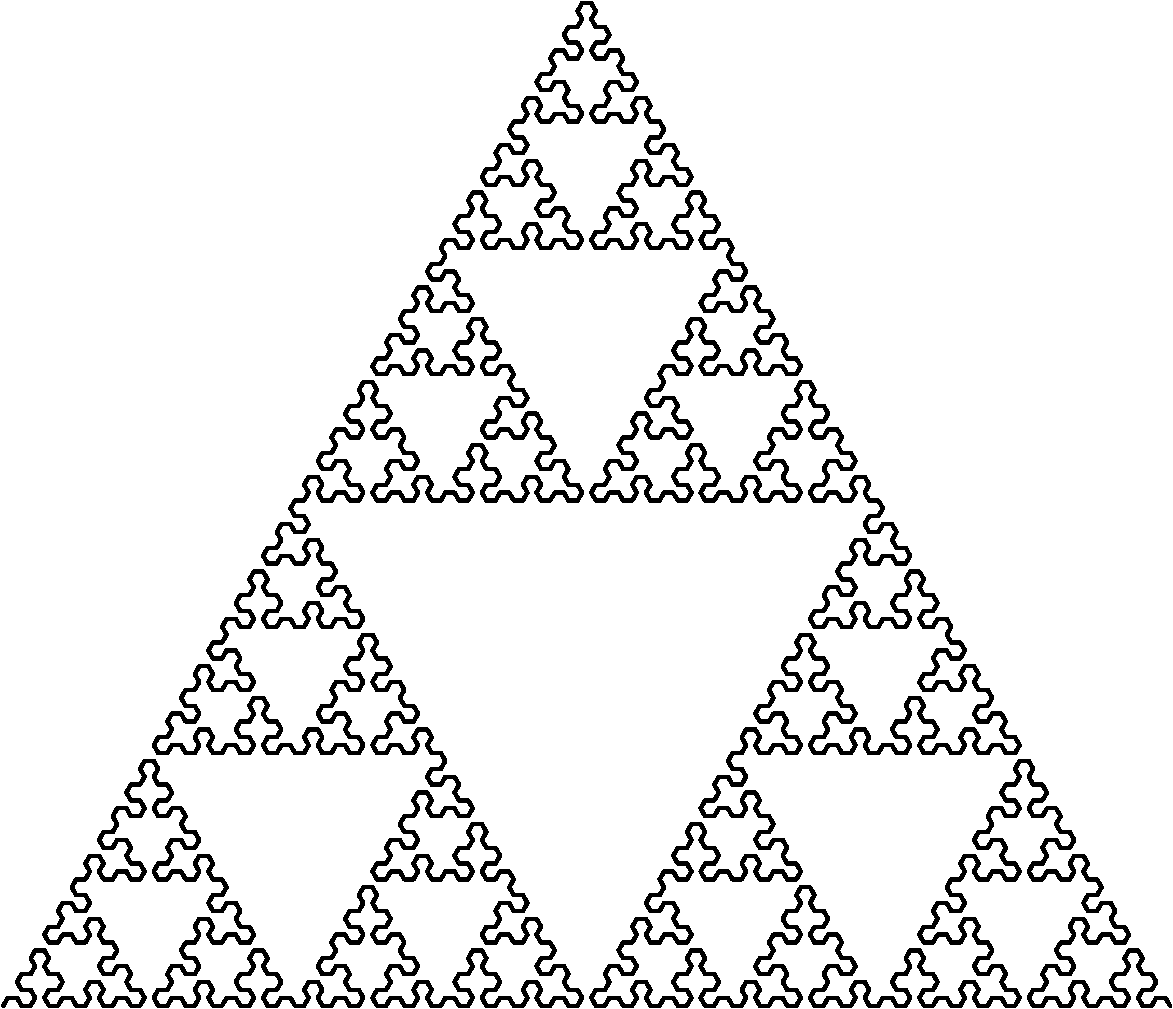
\includegraphics[width=\textwidth]{SierpinskiGasket}
		\endminipage
	}
	\caption{Example of source code along with the result -- Sierpinski gasket}
	\label{fig:scExample}
\end{figure}


\subsection{Source code compilation}

Source code compilation have two steps shown in Figure \ref{fig:compilePipeline}.
The first step is parsing of source code to \emph{abstract syntax tree} (further called AST).
Syntax parser will be generated by third-party parser generator (for details see section ??) which will guarantee robust and extensible syntax paring.
Each node of AST will contain information about position in original source code.
At this point AST can be used for syntax highlighting or source code formatting.

\begin{figure}[h]
	\centering
	\begin{tikzpicture}[auto, node distance=4cm,>=latex]
		\node (in) [coord] {};
		\node (yacc) [block, right of=in] {Lexer \& parser};
		\node (comp) [block, right of=yacc] {Compiler};
		\node (out) [coord, right of=comp] {};
		
		\draw [->] (in) -- node {source code} (yacc);
		\draw [->] (yacc) -- node {AST} (comp);
		\draw [->] (comp) -- node {semantic tree} (out);
	\end{tikzpicture}
	\caption{Source code compilation system}
	\label{fig:compilePipeline}
\end{figure}

Abstract syntax tree for source code \ref{lsys:ast} is shown in Figure \ref{fig:ast}.
You can see that expressions are not parsed as tree because operators (and their precedences) can be defined by user and will be processed by compiler in the next step.

\begin{Lsystem}[label=lsys:ast,caption={Constant definition statement for example of AST}]
let angle = 2 * random();
\end{Lsystem}

\tikzstyle{ast} = [draw, fill=blue!20, rectangle split, rectangle split parts=2, minimum height=2em]
\tikzstyle{astx} = [draw, fill=red!20, rectangle, rounded corners=1mm]

\begin{figure}[h]
	\centering
	\begin{tikzpicture}[child anchor=north,>=latex] %level/.style={sibling distance=33mm/#1},
		\node [ast] {Constant definition \nodepart{second} \footnotesize ln: 1, col: 1--25}
			[level distance=25mm, sibling distance=33mm]
			child { node [astx] {let} }
			child { node [ast] {Identificator \nodepart{second} \footnotesize ln: 1, col: 5--9}
				[level distance=14mm] child { node [astx] {angle} }
			}
			child { node [astx] {=} }
			child { node [ast] {Expression \nodepart{second} \footnotesize ln: 1, col: 13--24}
				[level distance=20mm, sibling distance=30mm]
				child { [level distance=14mm] node [ast] {Number \nodepart{second} \footnotesize ln: 1, col: 13} child { node [astx] {2} } }
				child { [level distance=14mm] node [ast] {Operator \nodepart{second} \footnotesize ln: 1, col: 15} child { node [astx] {*} } }
				child { [level distance=14mm] node [ast] {Function \nodepart{second} \footnotesize ln: 1, col: 17--24} child { node [astx] {random} } }
			}
			child { node [astx] {;} }
			;
	\end{tikzpicture}
	\caption{Abstract syntax tree of the statement \ref{lsys:ast}}
	\label{fig:ast}
\end{figure}

The next step of source code processing is compilation of AST into \emph{semantic tree} (further called ST).
Unlike AST semantic tree contains only data (no keywords or metadata about position).
However the nodes of semantic tree have reference to corresponding AST nodes to be possible to get the metadata for example for reporting locations of compilation errors.
Semantic tree in Figure \ref{fig:st} is created by compiling AST in Figure \ref{fig:ast}.
More complex semantic tree obtained from Source code \ref{lsys:stComplex} is shown in Figure \ref{fig:stComplex}.

\tikzstyle{st} = [draw, fill=blue!20, rectangle split, rectangle split parts=2, minimum height=2em]
\tikzstyle{stx} = [draw, fill=blue!20, rectangle, minimum height=2em]

\begin{figure}[h]
	\centering
	\begin{tikzpicture}[child anchor=north,>=latex] %level/.style={sibling distance=33mm/#1},
		\node [st] {Constant definition \nodepart{second} \footnotesize name: angle}
			[level distance=18mm, sibling distance=30mm]
			child { node [st] {Operator \nodepart{second} \footnotesize multiplication} 
				child { node [st] {Number \nodepart{second} \footnotesize 2} }
				child { node [st] {Function \nodepart{second} \footnotesize random} }
			}
			;
	\end{tikzpicture}
	\caption{Semantic tree of the AST on the figure \ref{fig:ast}}
	\label{fig:st}
\end{figure}


\begin{Lsystem}[label=lsys:stComplex,caption={Source code which results in more complex semantic tree \ref{fig:stComplex}}]
let iterBase = 2;
lsystem Octahedron {
	set symbols axiom = F;
	set iterations = iterBase + 1;
	interpret F as DrawForward(100, 2);
	interpret + as TurnLeft(45);
	rewrite F to F + F;
}
process all with SvgRenderer;
\end{Lsystem}

\begin{figure}[p]
	\centering
	\begin{tikzpicture}[grow'=right,child anchor=west,>=latex]
		\node [stx] {Input}
			[level distance=25mm, sibling distance=90mm]
			child { node [st] {Constant definition \nodepart{second} \footnotesize name: iterBase}
				[level distance=40mm]
				child {	node [st] {Number \nodepart{second} 2} }
			}
			child { node [st] {L-system \nodepart{second} \footnotesize name: Octahedron}
				[level distance=40mm, sibling distance=8mm]
				child { node [st] {Component property symbols assign \nodepart{second} \footnotesize name: axiom}
					[level distance=50mm]
					child { node [st] {Symbol \nodepart{second} F} }
				}
				child [missing] {}
				child [missing] {}
				child { node [st] {Component property assign \nodepart{second} \footnotesize name: iterations} 
					[level distance=43mm]
					child { node [st] {Operator \nodepart{second} \footnotesize addition} 
						[level distance=24mm, sibling distance=15mm]
						child { node [st] {Variable \nodepart{second} \footnotesize iterBase} }
						child { node [st] {Number \nodepart{second} \footnotesize 1} }
					}
				}
				child [missing] {}
				child [missing] {}
				child { node [st] {Interpretation \nodepart{second} \footnotesize name: DrawForward}
					[level distance=35mm, sibling distance=15mm]
					child { node [st] {Symbol \nodepart{second} F} }
					child { node [stx] {Parameters}
						[level distance=25mm]
						child {	node [st] {Number \nodepart{second} 100} }
						child {	node [st] {Number \nodepart{second} 2} }
					}
				}
				child [missing] {}
				child [missing] {}
				child [missing] {}
				child { node [st] {Interpretation \nodepart{second} \footnotesize name: TurnLeft}
					[level distance=35mm, sibling distance=15mm]
					child { node [st] {Symbol \nodepart{second} +} }
					child { node [stx] {Parameters}
						[level distance=25mm]						
						child { node [st] {Number \nodepart{second} 45} }
					}
				}
				child [missing] {}
				child [missing] {}
				child [missing] {}
				child [missing] {}
				child { node [st] {Rewrite rule \nodepart{second} \footnotesize symbol: F}
					[level distance=35mm, sibling distance=15mm]
					child { node [st] {Symbol \nodepart{second} F} }
					child { node [st] {Symbol \nodepart{second} +} }
					child { node [st] {Symbol \nodepart{second} F} }
				}
			}
			child { node [st] {Process statement \nodepart{second} \footnotesize L-system: all}
				[level distance=50mm]
				child { node [st] {Process configuration \nodepart{second} \footnotesize name: SvgRenderer} }
			}
			;
	\end{tikzpicture}
	\caption{More complex semantic tree of source code \ref{lsys:stComplex}}
	\label{fig:stComplex}
\end{figure}



\subsection{Input processing}
\label{sec:inputProcessing}

After compilation of input follows evaluation of input statements.
From evaluated statements are chosen \emph{process statements} which defines what \lsystem process with what component system.
Process manager will create appropriate component system, configure it and supply it all data needed for processing.
Then the control over processing is handed to component system and results are produced.
The processing of \lsystem is fully under control of component system.
Described procedure is shown in Figure \ref{fig:processPipeline}.

\begin{figure}[H]
	\centering
	\begin{tikzpicture}[auto, node distance=4cm,>=latex]
		\node (in) [coord] {};
		\node (eval) [block, right of=in] {Evaluator};
		\node (proc) [block, right of=eval, node distance=6cm] {Process manager};
		\node (compo) [coord, above of=eval, node distance=12mm] {};
		\node (compo2) [coord, above of=proc, node distance=12mm] {};
		\node (sys) [blockx, below of=proc, node distance=2cm] {Component system};
		\node (out) [coord, left of=sys] {};
		
		\draw [->] (in) -- node {semantic tree} (eval);
		\draw [->] (eval) -- node {evalued ST} (proc);
		\draw (compo) -- node {defined components} (compo2);
		\draw [->] (compo2) -- (proc);
		\draw [snakeline] (proc) -- node {} (sys);
		\draw [->] (sys) -- node {results} (out);
	\end{tikzpicture}
	\caption{Input processing scheme}
	\label{fig:processPipeline}
\end{figure}

All components will have access to \emph{process context}.
Process context will contain all properties of processed \lsystem, current components graph, output provider and some other data which can be user in processing.
Component can also provide values or functions to other components or to the user to use in input L-system (for example in rewrite rules or interpretation methods).  


\subsection{Measuring pass}
\label{sec:measuring}

Some components may need to know some information about processed model even if the model is not completed yet.
For example when some renderer component is producing image its dimensions are needed before any drawing can be done.
Also if we want to continuously color all lines with some gradient we must know total number of drawn lines.

The on way how component could achieve this is to cache all input and count needed metadata and after all input is supplied produce the output.
However this approach rises complexity of components and it can lead to significantly increased memory demands.
Caching also prevents communication between components about current state of \lsystem.
Imagine that some renderer wants to communicate with rewriter about rewriting style and some component in their way cahces all data .
In the time when renderer starts to render image rewriter already did all rewriting.

The library uses another way how to allow components to pre-count some metadata.
It is called \emph{measure pass}.
If any component needs to pre-count some metadata the Process manager invokes processing of whole system two times.
First pass is the \emph{measure pass} where all components can count metadata and no output is produced.
Second pass is ordinary processing of \lsystem but components already have metadata counted.
This way do not prevent communication between components about current state of \lsystem.

It is important to ensure that both passes will be equal.
For example problems can cause if component is using random generator for randomizing process.
Library provides unified approach for random numbers generation with \emph{Random provider} component.
Pseudo-random generator of the Random provider is resetted after each pass to the same value.
If the value of random seed is not provided by user it is generated randomly but it will be the same for both passes.
Concrete value of generated seed is supplied to user via message system to be possible to reproduce the output.

Figure \ref{fig:measurePassExample} demonstrates usage of measure pass with continuous coloring of line segments with rainbow gradient of \lsystem \ref{lsys:measurePassExample}.
Axiom of \lsystem is equilateral triangle.
In every iteration rewrite rule rewrites every line segment to line segment with triangle or square on it with the same probability 50\%.
Effect of the "triangle" part of rewrite rule is shown in sub-figures \ref{fig:measurePassExampleT1} and \ref{fig:measurePassExampleT2},
	effect of the "square" part is shown in \ref{fig:measurePassExampleR1} and \ref{fig:measurePassExampleR2}.
Result is randomized combination of previous.
First three and fifth iterations of \lsystem \ref{lsys:measurePassExample} are in sub-figures \ref{fig:measurePassExample1}, \ref{fig:measurePassExample2}, \ref{fig:measurePassExample3} and \ref{fig:measurePassExample5} respectively.

Notice that even that number of colored lines of \lsystem in Fig. \ref{fig:measurePassExample5} is random the rainbow gradient is applied correctly.
It is because in measure pass number of lines was counted and total sum was used in next pass to distribute gradient correctly.



\begin{Lsystem}[label=lsys:measurePassExample,caption={Stochastic \lsystem with variable number of line segments}]
lsystem WeirdKochCurve {
	set symbols axiom = F +(-120) F +(-120) F;
	set iterations = 5;
	set randomSeed = 2;
	set continuousColoring = true;

	interpret F as DrawForward(2 ^ -(currentIteration * 3/2) * 300);
	interpret + as TurnLeft;

	rewrite F
		to F +(60) F     +(-120)     F +(60) F  // triangle
		to F +(90) F +(-90) F +(-90) F +(90) F; // square
}
process all with SvgRenderer;
\end{Lsystem}

\begin{figure}[p]
	\centering
	\subfloat[Triangles 1st]{
\includegraphics[scale=0.3]{MeasurePassT1}\label{fig:measurePassExampleT1}} ~
	\subfloat[Triangles 2nd]{
\includegraphics[scale=0.3]{MeasurePassT2}\label{fig:measurePassExampleT2}} ~
	\subfloat[Rectangles 1st]{
\includegraphics[scale=0.3]{MeasurePassR1}\label{fig:measurePassExampleR1}} ~
	\subfloat[Rectangles 2nd]{
\includegraphics[scale=0.3]{MeasurePassR2}\label{fig:measurePassExampleR2}}
	\\
	\subfloat[Stochastic 1st iter.]{
\includegraphics[scale=0.4]{MeasurePass1}\label{fig:measurePassExample1}} ~
	\subfloat[Stochastic 2nd iter.]{
\includegraphics[scale=0.4]{MeasurePass2}\label{fig:measurePassExample2}} ~
	\subfloat[Stochastic 3rd iter.]{
\includegraphics[scale=0.4]{MeasurePass3}\label{fig:measurePassExample3}}
	\\
	\subfloat[Correctly colored 5th iteration of stochastic \lsystem]{
\includegraphics[scale=0.45]{MeasurePass5}\label{fig:measurePassExample5}}
	\caption{Example of stochastic \lsystem which is correctly colored by color gradient even if total number of colored line segments is random}
	\label{fig:measurePassExample}
\end{figure}

\subsection{Utilities}

Library will contain many useful functionality especially for components.

One large part will be functions for work with 3D.
The most important will be utility for triangulation of 3D objects defined by perimeter (3D version of polygons in 2D).
It should be able to triangulate any object in space but triangulation of 3D objects defined by perimeter is ambiguous so triangulation strategy will be configurable.
Part of 3D utilities will be functions for manipulation with points and vectors and quaternions.

Next utility will be for source code printing.
It will be capable to print and format abstract syntax tree as well as semantic tree.

























